\section{Model-Based Statistical Analysis} \label{sec:confirmatory}
Given the longitudinal nature of the study, in addition to considering the effect that the month and treatment variables have on reducing the level of mental distress across all participants, it is also important to address the correlation among the GSI scores obtained from each individual participant. The mixed-effects model is one of the most popular for analyzing longitudinal data for its intuitiveness and high interpretability. Particularly, it handles the individual-specific correlation by adding additional parameters at the individual level. Since the response (GSI) is continuous, and we have both continuous (month, education) and categorical (treatment, gender) explanatory variables, a natural model of choice is the linear mixed-effects model.\\\\
The linear mixed-effects model takes on the following general form:
\begin{align}
y_{ij} = (\beta_0 + b^0_i) + (\beta_1 + b^1_i)t_{ij} + (\beta_2 + b^2_i)x^2_i + \cdots + (\beta_n + b^n_i)x^n_i + e_{ij}. \label{eq:lme}
\end{align}
In our case, $y_{ij}$ denotes the GSI score of the $i$th participant at the $j$th time point. $t_{ij}$ represents the month variable for the $i$th participant at the $j$th time point. $x^2_i,\cdots,x^n_i$ correspond to the other explanatory variables that do not change over time for the $i$th participant. Finally the $e_{ij}$ terms are the residuals, which are assumed to be normally distributed and centred at $0$.\\\\
By fixing $j$ and ignoring the $b_i$ terms, we recover the familiar linear regression model, where the $\beta$ terms represent the effects of each explanatory variable on the response. By varying the time points $j$, we are able to model the effects of each explanatory variable considering the changes in the response over time. Including the $b_i$ terms allows the individual-specific correlation to be taken into consideration. The $b_i$ terms are the random effects. It is assumed that for each $k, b_i^k\sim N(0, \sigma^2_k)$ across all $i$.\\\\
Both of the questions that we would like to answer can be analyzed using different linear mixed-effects models. Specifically, by looking at the participants in the intervention group and the control group separately, the effect of the month variable on the GSI scores describes how mental distresses in each of the groups change over time. At the same time, by looking at both groups together, we can quantify the effect of mental health intervention by inspecting the $\beta$ term associated with the treatment variable. As a result, for the remainder of this section, we present in detail the analysis procedure that addresses whether mental distress decreases over time in the intervention group as an example. The analysis results addressing both of our main questions are carefully discussed in \cref{sec:analysis.results}.\\\\
Before proceeding to selecting the appropriate linear mixed-effects models that address our main objectives, it is worth noting that all of the entries that contain missing values, either on the explanatory variables or the response, are removed before conducting the following analysis. In addition, all of the participants with only one recorded GSI score are also excluded from the analysis below. This is because in such cases, there is no information on how the participant's mental distress has changed over time. Under the linear mixed-effects models, the removal of such observations implies that we are imposing the additional assumption that the reasons these values are missing do not depend on the missing values themselves. The missing values are more carefully treated in \cref{sec:handling.missing.data}.
\subsection{Model Selection}
\begin{wraptable}{r}{0.5\textwidth}
\resizebox{\linewidth}{!}{
\begin{tabular}{|l|l|l|}
\hline
& month & month/gender/education \\
\hline
month/gender & 0 & 0.016 \\
\hline
month/education & 0.004 & 0 \\
\hline
\end{tabular}
}
\caption{P values of Likelihood Ratio tests between models with different covariates under the intervention group}
\label{tab:model.comp.treatment.lrt}
\end{wraptable}
From \cref{eq:lme}, it is clear that setting any of the $\beta$'s to 0 implies the corresponding explanatory variable is not included in the linear mixed-effects model. At the same time, setting any set of $b_i^k$'s across all $i$ to 0 means that the random effects associated with the corresponding explanatory variable are not considered. A natural next step is then to identify the covariates and mixed effects that we would like to include in the model. By \cite{wu2009mixed}, common model selection metrics such as the AIC, BIC, and the p-values from likelihood ratio tests (LRT) can be employed. Both the AIC and BIC try to find the balance between goodness-of-fit and model complexity. In our case, since the total number of explanatory variables considered is not large, we are not overly concerned with model complexity. Therefore, we use the p-values from LRT to select an appropriate model to answer whether the mental distresses decrease over time among participants in the intervention group. The LRT tests whether one model is a significantly better fit than the other between two nested models. By nested models, we mean that the parameters of the smaller model form a subset of those of the larger model.\\\\
We begin by selecting the explanatory variables to be included in the model. Since we're interested in the changes of mental distress over time, the month variable must be included. From \cref{sec:eda}, we know that it is possible that one of the gender and education variables can explain much of the variabilities among the GSI scores. Therefore we compare the goodness-of-fit among models that include varying covariates using the LRT. The p-values are summarized in \cref{tab:model.comp.treatment.lrt}. Note that none of the mixed effects is considered here. In \cref{tab:model.comp.treatment.lrt}, the first column shows there is strong evidence (p-values $<0.004$) that including either of the gender or education variables leads to a better fit model. Then the second column shows there is moderate to strong evidence (p-values $<0.016$) including both covariates leads to a better fit model compared to those that only include one. As a result, we do not discard any of the covariates when studying the change in mental distress among participants in the intervention group. Similarly, as shown in \cref{app:cov.control,app:cov.both}, none of the covariates is discarded. Note that in \cref{app:cov.both}, the treatment variable is also included automatically because its effect is essential to detecting any effect of mental health intervention.\\
\begin{figure}[t]
\begin{subfigure}{.33\textwidth}
  \centering
  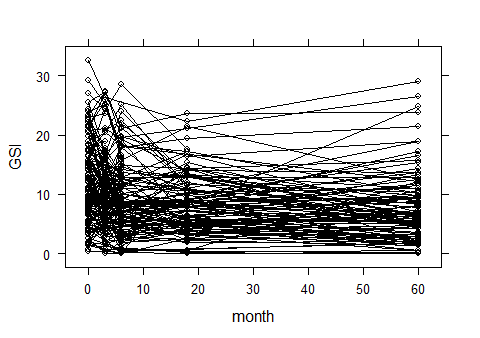
\includegraphics[width=1\linewidth]{../../plots/trellis_treatment.png}
  \caption{trellis plot of all subjects in the intervention group}
  \label{fig:4a}
\end{subfigure}
\begin{subfigure}{.33\textwidth}
  \centering
  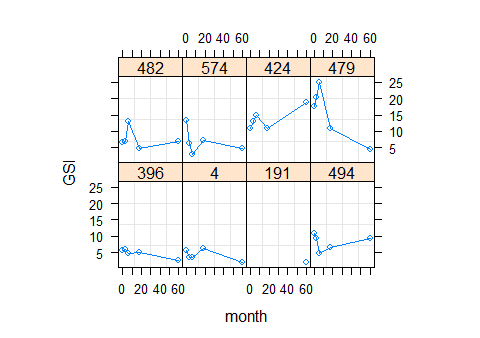
\includegraphics[width=1\linewidth]{../../plots/trellis_subset_treatment.png}
  \caption{trellis plot of randomly selected subjects}
  \label{fig:4b}
\end{subfigure}
\begin{subfigure}{.33\textwidth}
  \centering
  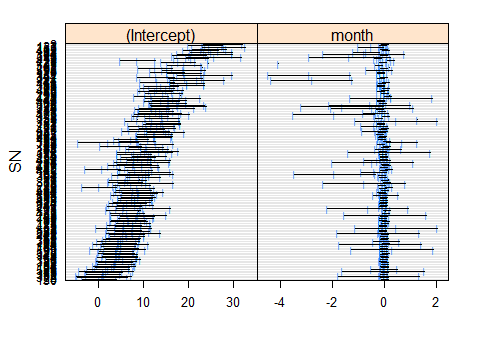
\includegraphics[width=1\linewidth]{../../plots/interval_treatment.png}
  \caption{confidence intervals of parameters from individual linear models}
  \label{fig:4c}
\end{subfigure}
\caption{Diagnostic plots for selection of random effects for the intervention group}
\label{fig:diagnostic.treatment}
\end{figure}

\noindent Now that the covariates to be included are determined for each model, the random effects can be selected following the same approach. The random effects allows us to adjust the effect that a explanatory variable or the intercept has for each participant on top of the overall average effect. Before formally deciding which random effects are to be included using the LRT, we use the plots in \cref{fig:diagnostic.treatment} to gauge whether the inclusion of any random effects is warranted.\\
\begin{wraptable}{r}{0.5\textwidth}
\resizebox{\linewidth}{!}{
\begin{tabular}{|l|l|l|l|}
\hline
& no mixed effect & intercept & intercept/month \\
\hline
intercept & 0 &/ &/ \\
\hline
intercept/month &/ & 0.028 &/ \\
\hline
intercept/gender &/ & 0.784 &/ \\
\hline
intercept/education &/ & 0.998 &/ \\
\hline
intercept/month/gender & /&/ & 0.893 \\
\hline
intercept/month/education & /&/ & 0.995 \\
\hline
\end{tabular}
}
\caption{P values of Likelihood Ratio tests between models with different mixed effects under the intervention group}
\label{tab:model.comp.treatment.me.lrt}
\end{wraptable}
\noindent By \cref{fig:4a}, it is clear that at the beginning of the study, the participants' levels of mental distresses are quite different in the intervention group. To better assess how the GSI scores change over time, we randomly select some of the participants and show how their GSI scores change over the course of the study in \cref{fig:4b}. While many of the participants' GSI scores exhibit an overall flat trend, there are participants whose GSI scores show clear increasing or decreasing trends acorss time. To better access the trends across time among all participants in the intervention group, we fit linear regression models without random effects on each of the participants' GSI scores individually and plot the 95\% confidence intervals of the regression parameters in \cref{fig:4c}. This plot verifies the variability present in the GSI scores at the beginning of the study as many of the confidence intervals of the individual intercepts do not overlap. While most confidence intervals of the individual regression parameters for the month variable hover around 0, we do have two instances where the confidence intervals are much different than the rest. These plots suggest that a random effect term is necessary for both the intercept and the month variable.\\\\
It is important to note, though, that each participant's gender and education variables do not change over the course of the study. Therefore when fitting individual linear regression models on each of the participants, the effect of the gender and education variables cannot be distinguished from the intercept. As a result, we only know that a random effect term is necessary for some of the intercept and the gender and education variables. To formally decide where to place the random effects among the intercept and the two covariates, we again use the p-values from the LRT.\\\\
As shown in \cref{tab:model.comp.treatment.me.lrt}, a stepwise procedure is used when comparing models that contain different random effect terms. We first note that adding a random effect term on the intercept leads to better fit model (p-value $\approx 0$). Then among the three covariates, there is moderate evidence that adding a random effect on the month variable leads to a better fit (p-value = 0.028). Finally, there is no evidence against that further including random effects on either gender or education results in the same level of goodness-of-fit (p-values $>0.893$). Therefore, when studying the changes in mental distress over time in the intervention group, a model that includes random effects on the intercept and the month variable is most appropriate.\\\\
Following the same procedure, as shown in \cref{app:re.control}, a random effect term is only added to the intercept term when studying the changes in mental distress over time in the control group. In \cref{app:re.both}, we see that random effect terms are added to both the intercept and the month variable.
\subsection{Assumption Check}
Before presenting the analysis results from the linear mixed-effects models selected above, recall that there are two distributional assumptions. Particularly, both the residuals and the random effects corresponding to each explanatory variable are assumed to be normally distributed with mean 0. Again as an example, we check whether these assumptions hold for the case of studying the changes in mental distress in the intervention group using the plots in \cref{fig:residual.treatment}.\\\\
\cref{fig:5a} shows the scatter plot between the fitted values and the residuals. Similar to \cref{sec:eda}, p-values from the t-test and Wilcoxon test quantifying the evidence against that the mean of the residuals is 0 are shown in the caption. We see that residuals seem to have a mean of 0. \cref{fig:5b} shows the residual QQ plot. If the residuals were indeed normally distributed, the dots in the plot should follow the slanted line closely. We see that this is clearly not the case for the larger residuals. This indicates that the normality assumption on the residuals may not hold. The QQ plots for both groups of the mixed effects are shown in \cref{fig:5c,fig:5d}. Similar to that of the residuals, while there is no evidence against that the means are 0 (p-values $> 0.335$), the normality assumptions seem to be violated. Overall, it seems like the normality assumptions of the linear mixed-effects model do not hold. This is also the case for the models investigating the changes in mental distress over time in the control group and the effectiveness of the treatment (\cref{app:assumption.check}). Therefore, we run the risk of drawing misleading conclusions if we draw conclusions only based off this set of linear mixed-effects models.\\\\
It is important to note that the normality assumption violations seem to be caused by a good portion of the responses rather than a small fraction of outliers. A common remedy in this case is to apply a log transformation of the response variables. However, this does not seem to help with the current set of data.
\begin{figure}[H]
\centering
\begin{subfigure}{.24\textwidth}
  \centering
  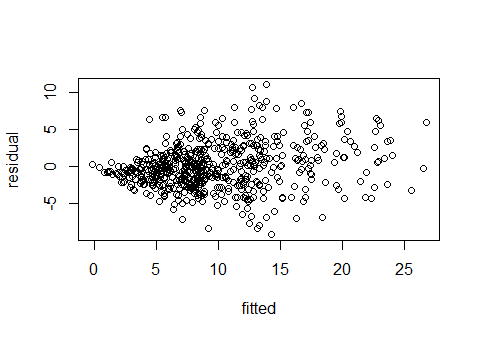
\includegraphics[width=1\linewidth]{../../plots/residual_treatment.png}
  \caption{fitted value vs. residual (t-test: 1, Wilcoxon: 0.204)}
  \label{fig:5a}
\end{subfigure}
\begin{subfigure}{.24\textwidth}
  \centering
  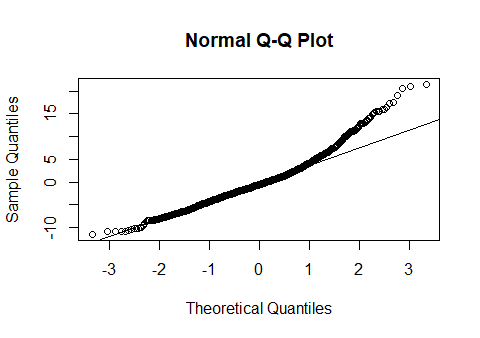
\includegraphics[width=1\linewidth]{../../plots/qq_residual_treatment.png}
  \caption{residual QQ plot}
  \label{fig:5b}
\end{subfigure}
\begin{subfigure}{.24\textwidth}
  \centering
  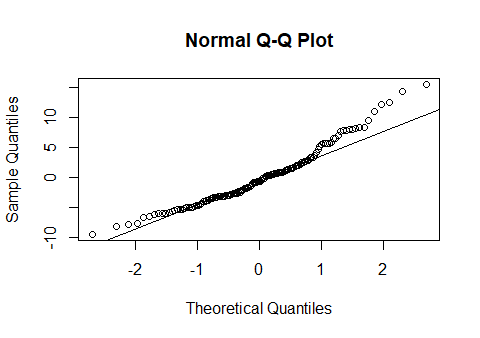
\includegraphics[width=1\linewidth]{../../plots/qq_intercept_treatment.png}
  \caption{QQ plot for the random effects on the intercept (t-test: 1, Wilcoxon: 0.335)}
  \label{fig:5c}
\end{subfigure}
\begin{subfigure}{.24\textwidth}
  \centering
  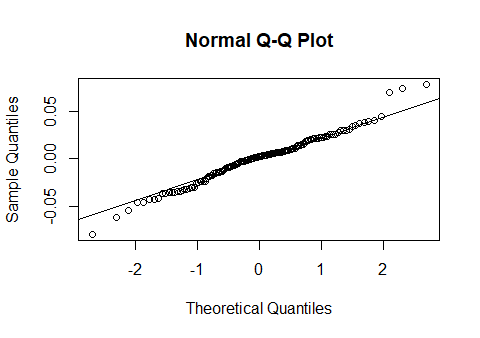
\includegraphics[width=1\linewidth]{../../plots/qq_slope_treatment.png}
  \caption{QQ plot for the random effects on the slope (t-test: 1, Wilcoxon: 0.781)}
  \label{fig:5d}
\end{subfigure}
\caption{Visualizing the residuals and random effects of the LME model under the intervention group}
\label{fig:residual.treatment}
\end{figure}
\noindent As a result, in addition to the linear mixed-effects models, a set of Generalized Estimating Equation (GEE) models are also conducted. The GEE model is commonly considered a non-parametric alternative to the mixed-effects model in longitudinal analysis. While the GEE model does not allow for individual-specific inference, there is no distributional assumptions that need to be satisfied for the model to produce reliable results. The GEE model under the linear model framework can be thought of as a generalization to the least squares method for estimating the regression parameters, which directly finds the set of parameters that minimizes the residual sum of squares without imposing the normality assumption. The removal of the normality assumption makes the GEE model more robust against the residuals' deviation from the normal distribution. Therefore, by if the analysis results are consistent between the linear mixed-effects models and the GEE models, we know that the analysis results are more reliable.\\\\
Note that for the GEE models to hold with the missing data removed, we do require that the missing values are missing completely at random. In other words, the reason for missing depends on neither the missing value itself nor any of the other variables in the model. Again, without knowing whether this assumption holds, we check how sensitive our analysis results are to these missing values in \cref{sec:handling.missing.data}. Finally, as a required input for the GEE models, we need to specify a covariance structure of the responses. An unstructed covariance is selected in all of our models, which, as shown in the next section, provides very robust parameter estimates.
\subsection{Analysis results}\label{sec:analysis.results}
The outputs from both the linear mixed-effects model and the GEE model for studying the changes in mental distress over time in the intervention group are shown in \cref{tab:lme.treatment,tab:gee.treatment}. First we look at the output from the linear mixed-effects model. It is clear that there is strong evidence (p-value $\approx 0$) that the effect of the month variable on the GSI scores is not zero. Recall that the GSI scores have been scaled by a factor of $10$. This then means that, with all of the other variables held fixed, as time goes on by a month, on average the GSI scores of the participants in the intervention group decrease by 0.0047. Then over the course of the study (60 months), the average decrease in GSI in the intervention group is estimated to be $0.282$, again with the other variables held fixed. The corresponding 95\% confidence interval of this estimated decrease in GSI per month is $(0.0030, 0.0063)$. From \cref{tab:gee.treatment}, we see that the GEE model ouputs a similar set of results, indicating the conclusions drawn are reliable. Note that the naive and robust standard errors are similar for each estimated effect, indicating the pre-selected unstructured covariance structure yield robust estimates.\\\\
Similarly, by \cref{tab:lme.control,tab:gee.control}, we can draw a reliable conclusion that there is moderate evidence (p-value = 0.017) that the effect of the month variable on the GSI scores is not zero. Particularly, with all of the other variables held fixed, as time goes on by a month, on average the GSI scores of the participants in the intervention group decrease by 0.0020 (0.12 over the course of the study). The corresponding 95\% confidence interval of this estimated decrease is $(0.0004, 0.0036)$. Overall, we have found that the mental distresses of the participants in both the intervention group and the control group decrease over time, although the amount of decrease may be small on a monthly level. These results are consistent with the preliminary conclusions drawn in \cref{sec:eda}.\\
\begin{table}[b]
\begin{minipage}{0.5\textwidth}
\centering
\resizebox{\linewidth}{!}{
\begin{tabular}{|l|r|r|r|r|r|}
\hline
  & Value & Std.Error & DF & t-value & p-value\\
\hline
(Intercept) & 11.933 & 2.758 & 465 & 4.326 & 0.000\\
\hline
month & -0.047 & 0.008 & 465 & -5.671 & 0.000\\
\hline
gender2 & 2.764 & 0.925 & 141 & 2.990 & 0.003\\
\hline
education & -0.249 & 0.190 & 141 & -1.314 & 0.191\\
\hline
\end{tabular}
}
\caption{Output of Linear Mixed Model under the intervention group}
\label{tab:lme.treatment}
\end{minipage}
\hfill
\begin{minipage}{0.5\textwidth}
\centering
\resizebox{\linewidth}{!}{
\begin{tabular}{|l|r|r|r|r|r|}
\hline
  & Estimate & Naive S.E. & Naive z & Robust S.E. & Robust z\\
\hline
(Intercept) & 11.162 & 2.484 & 4.494 & 2.538 & 4.397\\
\hline
month & -0.047 & 0.010 & -4.477 & 0.008 & -5.852\\
\hline
gender2 & 2.827 & 0.834 & 3.391 & 0.869 & 3.253\\
\hline
education & -0.194 & 0.170 & -1.146 & 0.173 & -1.125\\
\hline
\end{tabular}
}
\caption{Output of GEE model under the intervention group}
\label{tab:gee.treatment}
\end{minipage}
\end{table}

\noindent\noindent It might have been noticed that the above conclusions appear to contradict with the fact that most of the 95\% confidence intervals of individually estimated effects of the month variable seem to cover both sides of zero (\cref{fig:4c,fig:6c}). However, we note that these individual confidence intervals are fit with no more than five observations each, and so the corresponding uncertainties may be unusually large. As we simultaneously consider all participants in each group, the uncertainty of the estimated effect on the month variable should decrease. This ultimately leads to a small yet significant effect of the month variable on the GSI scores, which is in fact consistent with \cref{fig:4c,fig:6c}.\\
\begin{table}[t]
\begin{minipage}{0.5\textwidth}
\centering
\resizebox{\linewidth}{!}{
\begin{tabular}{|l|r|r|r|r|r|}
\hline
  & Value & Std.Error & DF & t-value & p-value\\
\hline
(Intercept) & 19.235 & 4.151 & 308 & 4.634 & 0.000\\
\hline
month & -0.020 & 0.008 & 308 & -2.394 & 0.017\\
\hline
gender2 & 2.606 & 1.383 & 95 & 1.884 & 0.063\\
\hline
education & -0.822 & 0.273 & 95 & -3.015 & 0.003\\
\hline
\end{tabular}
}
\caption{Output of Linear Mixed Model under the control group}
\label{tab:lme.control}
\end{minipage}
\hfill
\begin{minipage}{0.5\textwidth}
\centering
\resizebox{\linewidth}{!}{
\begin{tabular}{|l|r|r|r|r|r|}
\hline
  & Estimate & Naive S.E. & Naive z & Robust S.E. & Robust z\\
\hline
(Intercept) & 19.267 & 3.433 & 5.613 & 3.229 & 5.967\\
\hline
month & -0.027 & 0.013 & -2.019 & 0.010 & -2.606\\
\hline
gender2 & 2.220 & 1.148 & 1.935 & 1.216 & 1.825\\
\hline
education & -0.809 & 0.225 & -3.596 & 0.203 & -3.994\\
\hline
\end{tabular}
}
\caption{Output of GEE model under the control group}
\label{tab:gee.control}
\end{minipage}
\end{table}
\begin{table}[b]
\begin{minipage}{0.5\textwidth}
\centering
\resizebox{\linewidth}{!}{
\begin{tabular}{|l|r|r|r|r|r|}
\hline
  & Value & Std.Error & DF & t-value & p-value\\
\hline
(Intercept) & 15.418 & 2.341 & 774 & 6.586 & 0.000\\
\hline
treatment2 & -0.193 & 0.731 & 238 & -0.264 & 0.792\\
\hline
month & -0.037 & 0.006 & 774 & -5.893 & 0.000\\
\hline
gender2 & 2.737 & 0.776 & 238 & 3.527 & 0.001\\
\hline
education & -0.516 & 0.157 & 238 & -3.295 & 0.001\\
\hline
\end{tabular}
}
\caption{Output of Linear Mixed Model}
\label{tab:lme}
\end{minipage}
\hfill
\begin{minipage}{0.5\textwidth}
\centering
\resizebox{\linewidth}{!}{
\begin{tabular}{|l|r|r|r|r|r|}
\hline
  & Estimate & Naive S.E. & Naive z & Robust S.E. & Robust z\\
\hline
(Intercept) & 14.685 & 2.046 & 7.176 & 2.053 & 7.154\\
\hline
treatment2 & -0.430 & 0.641 & -0.671 & 0.735 & -0.586\\
\hline
month & -0.039 & 0.008 & -4.666 & 0.006 & -6.040\\
\hline
gender2 & 2.693 & 0.680 & 3.961 & 0.716 & 3.763\\
\hline
education & -0.455 & 0.136 & -3.337 & 0.139 & -3.278\\
\hline
\end{tabular}
}
\caption{Output of GEE model}
\label{tab:gee}
\end{minipage}
\end{table}

\noindent\noindent To answer whether mental health intervention is effective in reducing the level of mental distress, we look at the outputs from the linear mixed-effects models and the GEE models, which include both groups of participants and also the treatment variable as an additional explanatory variable. Note that since treatment variable is binary and that the intervention group is used as the baseline. Therefore the estimated effects of the treatment in \cref{tab:lme,tab:gee} describe the average difference in GSI scores in the control group when compared against the intervention group with the other variables held fixed. We see from \cref{tab:lme} that there is no evidence (p-value = 0.792) against that the average GSI scores are the same across the two groups with all other variables held fixed. In fact, the 95\% confidence interval of this estimated difference in GSI between the two groups, with the other variables held fixed, is $(-16.34, 12.48)$ (again recall the GSI scores have been scaled by a factor of 10). This means that mental health intervention do not appear to have a significant effect in reducing the level of mental distress.\\\\
From \cref{tab:gee}, we note that the GEE model's estimated effect on the treatment variable is about twice of that from the linear mixed-effects model. However, with standard errors at least as large as $0.641$, the corresponding 95\% confidence interval still covers both sides of zero, indicating there is no clear evidence against that the treatment effect is zero. Therefore, the conclusions drawn above is still reliable. Finally we note that this is also consistent with the preliminary conclusions from \cref{sec:eda}.
\subsection{Handling Missing Data} \label{sec:handling.missing.data}

\cite{little2019statistical}